% ============================================================================
%  Corridas de ejemplo, experimentos 0x02 y conclusiones
% ============================================================================
\newcommand{\EfitUs}{189}\newcommand{\EfitR}{0.92}\newcommand{\EfitB}{-0.10}\newcommand{\EfitCpuUs}{861}


\section{Corridas de ejemplo}\label{sec:corridas}

Se muestran tres corridas de cada caso, con la salida tal como la produce el programa
(las solicitudes se alimentaron por la entrada estándar, por eso la Box repite cada línea
leída). Las salidas completas están en la carpeta \texttt{runs/} del repositorio; las dos
más largas se recortaron aquí, conservando el inicio y el final.

\subsection{Caso A con dificultad indicada por el usuario}

Tres solicitudes con dificultades 95, 60 y 30 y duración aleatoria. La primera la resuelve
la raíz sola ($d>85$). En la segunda ($45<d\le85$) la raíz falla su Tiro Meeseeks, invoca 2
ayudantes con la dificultad diluida (de 60 a 75.67 y 72.21) y uno de ellos acierta; la
raíz detiene al resto del árbol e informa quién resolvió. En la tercera ($d\le45$) se
invocan 5 ayudantes y el árbol llega al nivel 3. Se observan los mensajes de bienvenida
con la tupla $(pid, ppid, N, i)$, los avisos por pipe, las despedidas recursivas y el
informe final de la Box.

\lstinputlisting[style=salida]{corridas/caso_A_texto.txt}

\subsection{Caso A con la dificultad a la suerte del Meeseeks}

El usuario presiona Enter en ambas preguntas: la raíz estima su dificultad con la
distribución Beta$(4,2)$ y la duración es aleatoria. En el informe final de la Box, el
asterisco junto a la dificultad indica que fue elegida al azar.

\lstinputlisting[style=salida]{corridas/caso_A_suerte.txt}

\subsection{Caso A imposible y plan de contingencia}

Una solicitud con $d=0$ y un tope reducido de 60 Meeseeks (\texttt{-m 60}) para que la
salida sea legible. La dificultad no se diluye nunca, cada generación tarda más (factor de
desesperación) y, al alcanzar el tope, las hojas reportan que no pueden invocar más
ayudantes; la falla sube hasta la raíz y la solicitud se registra como no completada sin
que el sistema colapse.

\lstinputlisting[style=salida]{corridas/caso_A_imposible.txt}

\subsection{Caso B: cálculos}

Tres expresiones: una aritmética, una lógica y una con división entre cero. La segunda es
interesante: $\sqrt2\cdot\sqrt2$ no es exactamente 2 en punto flotante
($2.0000000000000004$), así que la igualdad vale 0; aun así la expresión completa es
verdadera por la disyunción. La tercera se reporta como error y como solicitud no
completada.

\lstinputlisting[style=salida]{corridas/caso_B_calc.txt}

\subsection{Caso C: programas externos}

Tres programas: \texttt{ls} (código 0), una tubería con \texttt{gcc --version} (código 0) y un
comando inexistente, que el intérprete reporta con el código 127 y por lo tanto queda como
no completado.

\lstinputlisting[style=salida]{corridas/caso_C_run.txt}

\subsection{Caos planetario}

Una tarea imposible con el tope desactivado en la práctica (\texttt{-m 100000}) y un
tiempo máximo reducido a 20~s para la demostración. Al vencer el plazo la Box decreta el
caos, termina el grupo de procesos y cierra el programa con el informe. El experimento E6
estudia qué pasa si, en lugar de terminar, se deja seguir a los Meeseeks.

\lstinputlisting[style=salida]{corridas/caos_T20.txt}

% ===========================================================================
\section{0x02: experimentos y análisis}\label{sec:exp}

\subsection{Metodología}

Todas las mediciones se tomaron con el programa final, en una máquina virtual Linux
(kernel 6.18, 2 núcleos, 8~GB de RAM, \texttt{pid\_max} = 32\,768) y sin otra carga. Cada
experimento alimenta la Box por la entrada estándar en modo silencioso (\texttt{-q}), para
que el costo de imprimir en pantalla no contamine los tiempos, y guarda una fila CSV por
solicitud (\texttt{-o}). El script \texttt{experiments/run\_experiments.sh} reproduce
todos los experimentos y \texttt{experiments/analyze.py} genera las tablas y figuras de
esta sección directamente desde los CSV, sin transcribir números a mano. Los tiempos son
los definidos en la sección~\ref{sec:medidas}: $\Tt$, $\Ts$, $\Tr=\Tt-\Ts$ y CPU de los
descendientes.

Para que las comparaciones sean válidas, en cada experimento se cambia una sola variable y
el resto queda fijo. En los experimentos sobre la dificultad se usa una duración fija y
corta (0.1~s) en lugar de la aleatoria: así las diferencias se deben a la dificultad y no
al azar de las esperas, y se pueden repetir 20 veces cada caso en tiempos razonables. La
duración aleatoria se estudia aparte en E2.

\begin{center}
\begin{tabularx}{\linewidth}{lXl}
\toprule
Exp. & Pregunta & Variable \\
\midrule
E1 & ¿Cómo crece el costo con la dificultad? ¿Cuánto cuesta cada Meeseeks? & $d$ (22 valores, 20 rep.) \\
E2 & ¿Qué efecto tiene que la duración sea aleatoria y no fija? & duración (10 rep.) \\
E3 & ¿Cuánto cuesta en tiempo real cada caso (A, B y C)? & tipo de solicitud \\
E4 & ¿Qué efecto tienen las capas del plan de contingencia? & \texttt{-a}, \texttt{-m} \\
E5 & ¿Qué tan sensible es el modelo a la ganancia de dilución? & $g$ \\
E6 & ¿Cuánto tiempo extra necesita una tarea que supera el máximo? & $d$ muy pequeña, \texttt{-x} \\
\bottomrule
\end{tabularx}
\end{center}

\subsection{E1: costo en función de la dificultad}

Se enviaron 20 solicitudes de texto por cada uno de 22 valores de dificultad, con
duración fija de 0.1~s y la configuración por defecto (128 \emph{slots}, tope de 3000).

\begin{table}[H]
\centering\small
\begin{tabular}{rrrrrrrrrr}
\toprule
$d$ & Éxito & Meeseeks & RIC & Máx. & Niv. & $T_{total}$ & $T_{sim}$ & $T_{real}$ & CPU \\
\midrule
100 & 100\,\% & 1 & 1--1 & 1 & 1 & 0.101 & 0.10 & 0.0008 & 0.0005 \\
95 & 100\,\% & 1 & 1--1 & 1 & 1 & 0.101 & 0.10 & 0.0009 & 0.0005 \\
90 & 100\,\% & 1 & 1--1 & 1 & 1 & 0.101 & 0.10 & 0.0008 & 0.0004 \\
86 & 100\,\% & 1 & 1--1 & 1 & 1 & 0.101 & 0.10 & 0.0008 & 0.0004 \\
85 & 100\,\% & 2 & 1--3 & 3 & 2 & 0.156 & 0.15 & 0.0014 & 0.0010 \\
80 & 100\,\% & 1 & 1--3 & 5 & 1 & 0.101 & 0.10 & 0.0010 & 0.0005 \\
70 & 100\,\% & 3 & 1--5 & 5 & 2 & 0.212 & 0.21 & 0.0019 & 0.0017 \\
60 & 100\,\% & 5 & 3--5 & 9 & 3 & 0.212 & 0.21 & 0.0022 & 0.0024 \\
50 & 100\,\% & 5 & 5--8 & 11 & 3 & 0.215 & 0.21 & 0.0029 & 0.0026 \\
46 & 100\,\% & 8 & 5--11 & 13 & 4 & 0.333 & 0.33 & 0.0033 & 0.0030 \\
45 & 100\,\% & 10 & 8--14 & 18 & 3 & 0.213 & 0.21 & 0.0029 & 0.0039 \\
40 & 100\,\% & 12 & 8--16 & 26 & 3 & 0.213 & 0.21 & 0.0029 & 0.0043 \\
30 & 100\,\% & 14 & 12--22 & 31 & 3 & 0.214 & 0.21 & 0.0041 & 0.0056 \\
20 & 100\,\% & 68 & 54--71 & 75 & 4 & 0.342 & 0.33 & 0.0123 & 0.0243 \\
10 & 100\,\% & 140 & 127--174 & 283 & 4 & 0.355 & 0.33 & 0.0245 & 0.0417 \\
5 & 100\,\% & 288 & 280--304 & 321 & 5 & 0.507 & 0.46 & 0.0470 & 0.1125 \\
2 & 100\,\% & 316 & 292--458 & 540 & 5 & 0.513 & 0.46 & 0.0534 & 0.1246 \\
1 & 100\,\% & 494 & 460--639 & 686 & 6 & 0.691 & 0.60 & 0.0913 & 0.2526 \\
0.5 & 100\,\% & 652 & 630--768 & 825 & 7 & 0.873 & 0.75 & 0.1234 & 0.3797 \\
0.1 & 100\,\% & 1070 & 959--1097 & 1125 & 10 & 1.418 & 1.17 & 0.1828 & 0.7972 \\
0.01 & 100\,\% & 1581 & 1504--1627 & 1777 & 14 & 2.108 & 1.86 & 0.2764 & 1.4727 \\
0 & 0\,\% & 3000 & 3000--3000 & 3000 & 20 & 13.447 & 12.05 & 1.4006 & 14.1741 \\
\bottomrule
\end{tabular}

\caption{E1: medianas por dificultad (20 repeticiones). RIC es el rango intercuartílico de
los Meeseeks creados. Tiempos en segundos.}
\label{tab:e1}
\end{table}

\begin{figure}[H]
\centering
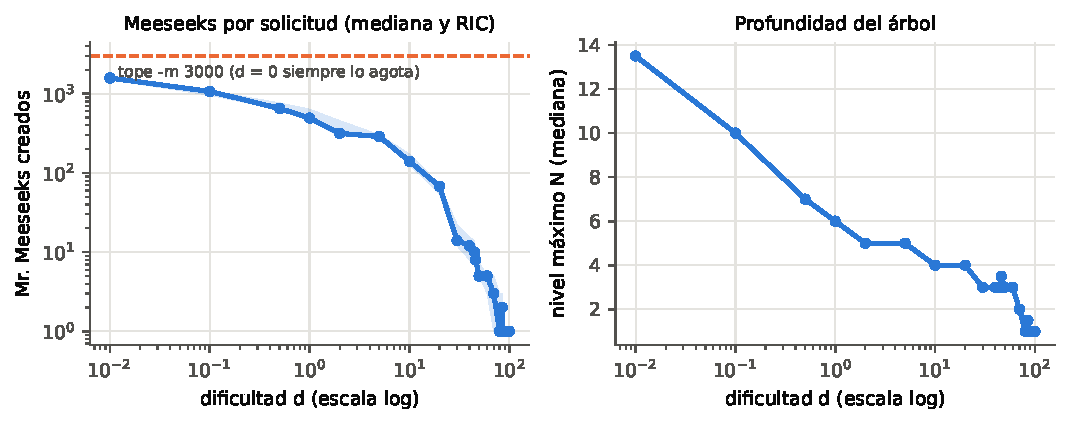
\includegraphics[width=\linewidth]{figs/e1_costo.pdf}
\caption{E1: Meeseeks creados y profundidad del árbol frente a la dificultad (ejes
logarítmicos en $d$; las solicitudes con $d=0$ no aparecen porque $\log 0$ no existe y
siempre llegan al tope).}
\label{fig:e1}
\end{figure}

\paragraph{Observaciones.}
\begin{itemize}[leftmargin=1.5em]
\item Para $d>85$ siempre basta un Meeseeks y $\Tt$ es prácticamente la duración
  simulada: el sistema operativo agrega menos de 1~ms.
\item Entre 45 y 85 se crean pocos Meeseeks (entre 1 y 13) gracias al Tiro Meeseeks y a
  que con 2 ayudantes la dificultad sube rápido. Se nota la discontinuidad del enunciado en
  $d=45$: con $d=46$ se piden 2 ayudantes y con $d=45$ se piden 5. Con 5 ayudantes se crean
  algo más de procesos (10 contra 8 en mediana), pero el árbol es menos profundo (3 contra
  4 niveles) y la tarea termina antes (0.213~s contra 0.333~s). Más paralelismo cambia
  procesos por tiempo.
\item Por debajo de $d\approx20$ el costo crece rápidamente: 68 Meeseeks con $d=20$, 288
  con $d=5$ y más de 1500 con $d=0.01$. Sin embargo, como la dilución multiplica la facilidad
  por casi 2.1 en cada generación, la profundidad solo crece como $\log(1/d)$: de 4 niveles
  con $d=10$ a 14 con $d=0.01$. El tiempo total sigue esa misma ley logarítmica.
\item Todas las tareas con $d>0$ se resolvieron (100\,\%). Todas las de $d=0$ terminaron
  en el tope de 3000 Meeseeks, con una mediana de 20 niveles, sin colapsar el sistema.
\end{itemize}

\begin{figure}[H]
\centering
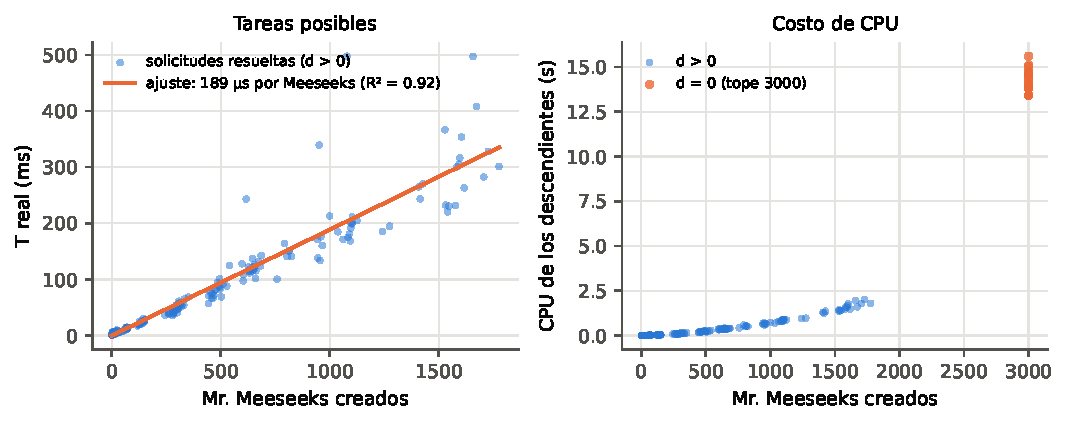
\includegraphics[width=\linewidth]{figs/e1_overhead.pdf}
\caption{E1: tiempo real (sin esperas simuladas) y CPU frente a la cantidad de Meeseeks
creados.}
\label{fig:e1b}
\end{figure}

\paragraph{Costo por Meeseeks.} En las solicitudes resueltas, el tiempo real crece de forma
lineal con la cantidad de Meeseeks: el ajuste da unos \EfitUs~µs de tiempo de pared por
Meeseeks ($R^2=\EfitR$) y unos \EfitCpuUs~µs de CPU. La CPU supera al tiempo de pared
porque hay dos núcleos trabajando en paralelo y porque cada \texttt{fork()} copia las tablas
de páginas del padre. En cambio, las tareas imposibles se salen de la recta (puntos naranja):
3000 Meeseeks consumen alrededor de 14~s de CPU, unas cinco veces lo que predice el
ajuste. La causa se analiza en E4.

\subsection{E2: duración aleatoria frente a duración fija}

Para tres dificultades se comparó la duración aleatoria uniforme en $[0.5, 5]$~s contra
una duración fija igual a su media (2.75~s), con 10 repeticiones cada una.

\begin{table}[H]
\centering\small
\begin{tabular}{rlrrrrr}
\toprule
$d$ & Duración & $T_{total}$ (s) & $T_{sim}$ (s) & $T_{real}$ (ms) & Meeseeks & Niv. \\
\midrule
90 & aleatoria 0.5-5 s & 2.90 $\pm$ 1.33 & 2.89 & 3.5 $\pm$ 1.4 & 1 & 1 \\
90 & fija 2.75 s & 2.75 $\pm$ 0.00 & 2.75 & 4.0 $\pm$ 1.5 & 1 & 1 \\
50 & aleatoria 0.5-5 s & 6.44 $\pm$ 2.00 & 6.43 & 8.2 $\pm$ 2.6 & 5 & 3 \\
50 & fija 2.75 s & 7.43 $\pm$ 1.74 & 7.42 & 9.7 $\pm$ 2.1 & 6 & 3 \\
20 & aleatoria 0.5-5 s & 5.53 $\pm$ 0.95 & 5.52 & 10.9 $\pm$ 3.5 & 28 & 4 \\
20 & fija 2.75 s & 8.43 $\pm$ 1.40 & 8.42 & 18.2 $\pm$ 5.6 & 63 & 4 \\
\bottomrule
\end{tabular}

\caption{E2: media $\pm$ desviación estándar; Meeseeks y niveles en mediana.}
\end{table}

\begin{figure}[H]
\centering
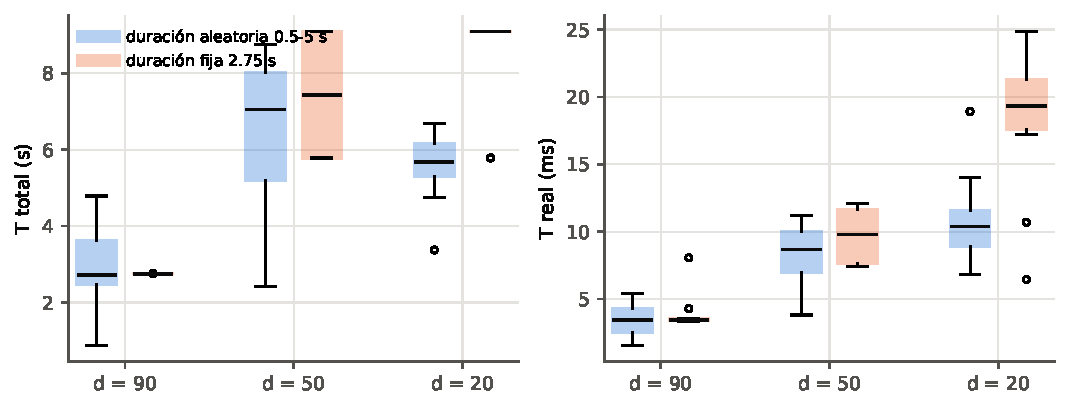
\includegraphics[width=\linewidth]{figs/e2_aleatorio.pdf}
\caption{E2: tiempo total y tiempo real según el tipo de duración.}
\end{figure}

\paragraph{Observaciones.}
\begin{itemize}[leftmargin=1.5em]
\item El tiempo total está dominado por completo por la espera simulada: $\Tt$ y $\Ts$
  difieren en milisegundos. Esto confirma que, para comparar el costo del sistema, hay que
  mirar $\Tr$ y no $\Tt$.
\item Con un solo Meeseeks ($d=90$) la media es la misma con ambas duraciones (2.90 contra
  2.75~s), como se espera, pero la aleatoria tiene una dispersión grande.
\item Con muchos Meeseeks ($d=20$) ocurre algo menos obvio: la duración aleatoria es
  \emph{más rápida} (5.53 contra 8.43~s) y crea menos de la mitad de los procesos (28 contra
  63). Cuando varias ramas trabajan en paralelo, la solución llega por la rama que
  terminó primero, y el mínimo de varias duraciones aleatorias es mucho menor que su media.
  Además, al resolverse antes, no alcanzan a nacer las generaciones siguientes. En la
  serie, un Meeseeks con suerte puede ahorrarle trabajo a todos los demás.
\item El tiempo real de un solo Meeseeks es de unos 3.5~ms tras dormir 2.75~s, mientras que
  en E1, tras dormir 0.1~s, era de 0.8~ms. La diferencia no viene del programa sino de la
  latencia para despertar: después de varios segundos de inactividad la máquina virtual
  pone a dormir los núcleos y reactivarlos cuesta algunos milisegundos.
\end{itemize}

\subsection{E3: comparación de los tres casos}

Se midió el tiempo real de cada tipo de solicitud que atiende un solo Meeseeks. Para el
caso A se usó $d=100$ con una duración de 1~µs, de modo que el tiempo medido sea
prácticamente solo el del mecanismo.

\begin{table}[H]
\centering\small
\begin{tabular}{lrrrrrr}
\toprule
Caso & n & Éxito & Media (ms) & Mediana (ms) & P95 (ms) & CPU (ms) \\
\midrule
A: texto d=100 (1 Meeseeks) & 200 & 100\,\% & 0.319 & 0.276 & 0.531 & 0.230 \\
B: calc (válido) & 150 & 100\,\% & 0.282 & 0.256 & 0.376 & 0.278 \\
B: calc (error) & 50 & 0\,\% & 0.253 & 0.230 & 0.407 & 0.254 \\
C: run true & 200 & 100\,\% & 2.400 & 2.332 & 2.851 & 2.253 \\
C: run false & 50 & 0\,\% & 2.133 & 2.019 & 2.721 & 2.135 \\
C: run ls /usr/bin & 50 & 100\,\% & 5.878 & 5.472 & 7.382 & 5.616 \\
C: run sleep 0.25 & 20 & 100\,\% & 255.429 & 255.288 & 256.103 & 4.929 \\
\bottomrule
\end{tabular}

\caption{E3: tiempo real por tipo de solicitud.}
\end{table}

\begin{figure}[H]
\centering
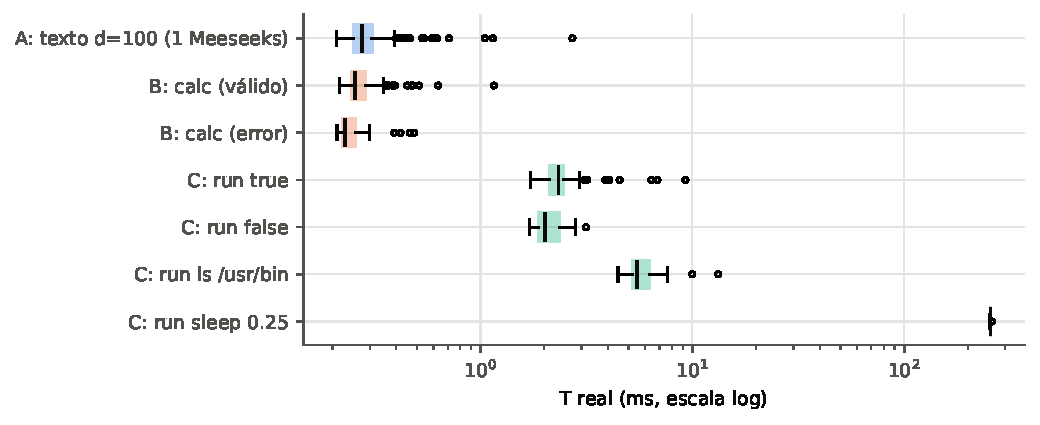
\includegraphics[width=\linewidth]{figs/e3_casos.pdf}
\caption{E3: distribución del tiempo real por caso (escala logarítmica).}
\end{figure}

\paragraph{Observaciones.}
\begin{itemize}[leftmargin=1.5em]
\item Los casos A (un Meeseeks) y B cuestan lo mismo, alrededor de 0.25 a 0.3~ms: ese es el
  costo base de crear un proceso con \texttt{fork()}, mandarle un mensaje por pipe, recibir
  la respuesta y recogerlo con \texttt{waitpid()}. Evaluar la expresión es despreciable
  frente a eso, y que la expresión tenga un error no cambia el tiempo.
\item El caso C es unas 9 veces más caro (unos 2.3~ms con \texttt{true}) porque el
  Meeseeks hace un segundo \texttt{fork()} y un \texttt{exec()} de \texttt{/bin/sh}, que a
  su vez carga y ejecuta el programa: cargar un ejecutable nuevo (abrir el archivo, mapear
  sus segmentos, enlazar bibliotecas dinámicas) cuesta mucho más que duplicar un proceso
  que ya está en memoria.
\item El resultado del programa externo no cambia el costo (\texttt{true} y \texttt{false}
  tardan lo mismo); lo que cambia es el trabajo del programa (\texttt{ls /usr/bin} tarda
  más del doble) y, sobre todo, si el programa espera: con \texttt{sleep 0.25} el tiempo
  real es de 255~ms, pero la CPU es de solo 5~ms. En el caso C no hay espera simulada, así
  que el tiempo del programa externo es tiempo real de la solicitud.
\end{itemize}

\subsection{E4: plan de contingencia}

\paragraph{E4a: semáforo de \emph{slots}.} Con $d=10$ y duración 0.1~s (15 repeticiones)
se varió la cantidad de Meeseeks que pueden trabajar a la vez.

\begin{table}[H]
\centering\small
\begin{tabular}{rrrrrrr}
\toprule
Slots (\texttt{-a}) & $T_{total}$ (s) & $T_{real}$ (ms) & Meeseeks & Pico vivos & Niv. & CPU (ms) \\
\midrule
2 & 0.605 & 5.0 & 9 & 9 & 5 & 10.0 \\
4 & 0.465 & 4.8 & 16 & 14 & 5 & 11.4 \\
8 & 0.467 & 6.7 & 28 & 24 & 5 & 16.1 \\
16 & 0.468 & 9.3 & 44 & 38 & 5 & 23.6 \\
32 & 0.343 & 12.9 & 66 & 59 & 4 & 24.9 \\
64 & 0.350 & 20.0 & 100 & 92 & 4 & 37.6 \\
128 & 0.353 & 22.7 & 142 & 133 & 4 & 44.3 \\
512 & 0.352 & 22.1 & 140 & 135 & 4 & 42.3 \\
\bottomrule
\end{tabular}

\caption{E4a: medianas según la cantidad de \emph{slots}.}
\end{table}

\begin{figure}[H]
\centering
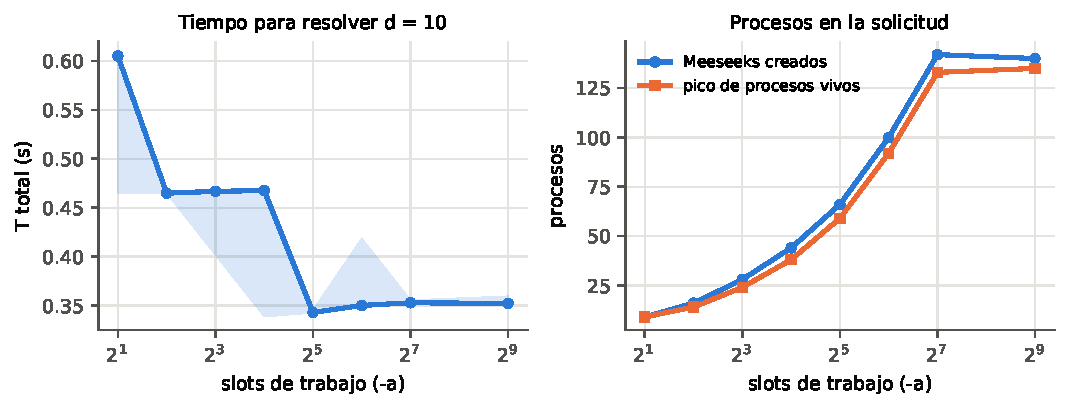
\includegraphics[width=\linewidth]{figs/e4a_slots.pdf}
\caption{E4a: efecto del semáforo de \emph{slots} con $d=10$.}
\end{figure}

Restringir los \emph{slots} reduce mucho los procesos creados (de 142 a 9) y la CPU (de
44 a 10~ms) a cambio de un poco más de tiempo (de 0.35 a 0.61~s). Con pocos \emph{slots}
el árbol crece en profundidad en lugar de en anchura: los primeros Meeseeks en conseguir
\emph{slot} siguen diluyendo la tarea hacia abajo, y cuando uno la resuelve todavía no han
nacido muchos de sus primos. Con muchos \emph{slots} se crean procesos que al final no
sirven. Por encima de 128 no hay diferencia porque el árbol nunca necesita más.

\paragraph{E4b: tope total con tareas imposibles.} Con $d=0$ y duración 0.1~s (5
repeticiones) se varió el tope \texttt{-m}.

\begin{table}[H]
\centering\small
\begin{tabular}{rrrrrrrr}
\toprule
Tope (\texttt{-m}) & Éxito & $T_{total}$ (s) & $T_{real}$ (s) & Meeseeks & Pico vivos & Niv. & CPU (s) \\
\midrule
100 & 0\,\% & 0.71 & 0.013 & 100 & 98 & 4 & 0.04 \\
250 & 0\,\% & 1.02 & 0.021 & 250 & 247 & 5 & 0.09 \\
500 & 0\,\% & 1.79 & 0.038 & 500 & 499 & 7 & 0.35 \\
1000 & 0\,\% & 3.89 & 0.040 & 1000 & 999 & 11 & 1.56 \\
2000 & 0\,\% & 8.57 & 0.071 & 2000 & 1999 & 17 & 6.01 \\
3000 & 0\,\% & 13.27 & 1.818 & 3000 & 2994 & 20 & 14.07 \\
5000 & 0\,\% & 29.52 & 14.569 & 5000 & 4951 & 23 & 44.30 \\
\bottomrule
\end{tabular}

\caption{E4b: medianas según el tope de Meeseeks para una tarea imposible.}
\end{table}

\begin{figure}[H]
\centering
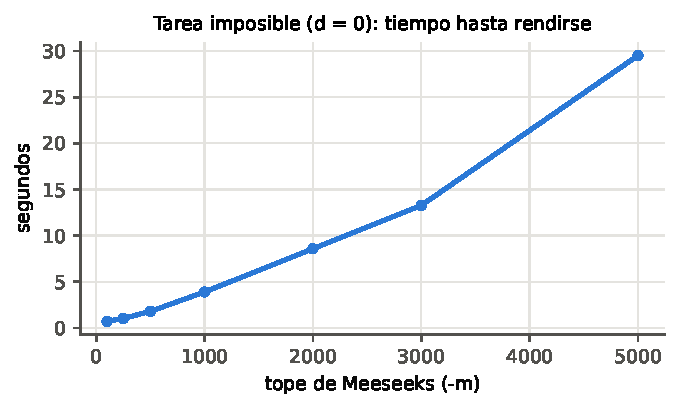
\includegraphics[width=0.62\linewidth]{figs/e4b_tope.pdf}
\caption{E4b: tiempo hasta rendirse frente al tope.}
\end{figure}

El tope cumple su función: ninguna tarea imposible pasó del límite y todas terminaron en
segundos. Sin embargo, el costo no es lineal en el tope. Al duplicar de 1000 a 2000
Meeseeks la CPU se multiplica por casi 4, y con 5000 el programa usó unos 44~s de CPU en
30~s de pared, es decir, los dos núcleos casi saturados. El pico de procesos vivos es
prácticamente igual al tope, porque en una tarea imposible casi nadie termina hasta que se
rinde todo el árbol.

La causa es una decisión de diseño. Un padre que quiere crear un ayudante y no encuentra
\emph{slot} no se bloquea en \texttt{sem\_wait}, porque necesita seguir atendiendo su pipe
(podría llegarle \texttt{M\_STOP}); en su lugar vuelve a intentarlo cada 25~ms con
\texttt{poll()}. Con miles de padres en esa situación, el sistema hace miles de intentos por
segundo y la cantidad de intentos crece con la cantidad de padres multiplicada por el tiempo
que esperan, lo que da un costo cuadrático. Es una forma de espera activa. Una mejora sería
que los Meeseeks que liberan un \emph{slot} despierten a los que esperan por un descriptor
(por ejemplo un pipe de fichas o un \texttt{eventfd}) que se pueda vigilar con el mismo
\texttt{poll()}; así la espera sería pasiva sin dejar de atender el pipe.

\subsection{E5: sensibilidad a la ganancia de dilución}

La ganancia $g$ controla qué tan rápido se simplifica la tarea entre generaciones. Se
probaron tres valores con tres dificultades (20 repeticiones, duración 0.1~s).

\begin{table}[H]
\centering\small
\begin{tabular}{rrrrrrrr}
\toprule
$d$ & $g$ & Éxito & Meeseeks (med.) & Máx. & Niv. & $T_{total}$ (s) & $T_{real}$ (ms) \\
\midrule
50 & 0.25 & 100\,\% & 11 & 29 & 4 & 0.333 & 3.1 \\
50 & 0.5 & 100\,\% & 5 & 13 & 3 & 0.212 & 2.3 \\
50 & 1 & 100\,\% & 5 & 7 & 3 & 0.212 & 2.0 \\
20 & 0.25 & 100\,\% & 136 & 268 & 4 & 0.351 & 21.0 \\
20 & 0.5 & 100\,\% & 65 & 77 & 4 & 0.340 & 10.4 \\
20 & 1 & 100\,\% & 14 & 24 & 3 & 0.213 & 3.1 \\
5 & 0.25 & 100\,\% & 488 & 635 & 6 & 0.676 & 76.1 \\
5 & 0.5 & 100\,\% & 285 & 371 & 5 & 0.504 & 44.0 \\
5 & 1 & 100\,\% & 114 & 135 & 4 & 0.348 & 17.3 \\
\bottomrule
\end{tabular}

\caption{E5: efecto de la ganancia $g$ (medianas).}
\end{table}

\begin{figure}[H]
\centering
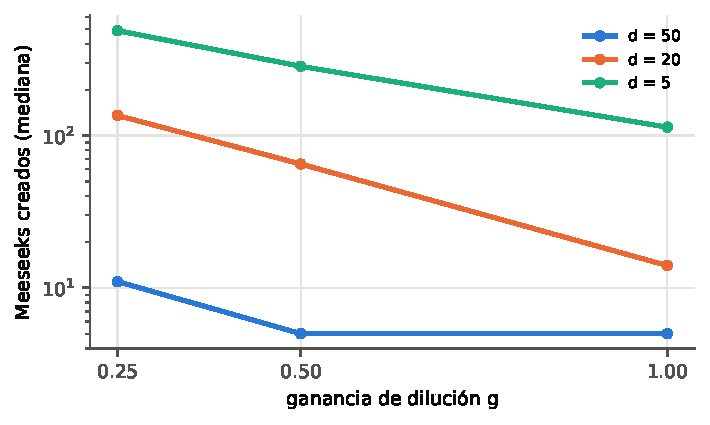
\includegraphics[width=0.66\linewidth]{figs/e5_ganancia.pdf}
\caption{E5: Meeseeks creados según la ganancia.}
\end{figure}

Con $g=1$ la dilución es tan rápida que incluso $d=5$ se resuelve con alrededor de 110
Meeseeks y 4 niveles; con $g=0.25$ se necesitan unos 490 y 6 niveles. El efecto es mayor para las
dificultades medianas ($d=20$: de 136 a 14 Meeseeks, casi diez veces menos) que para las
fáciles. El valor por defecto $g=0.5$ es un término medio: deja ver árboles grandes para
tareas difíciles, como en la serie, sin que las tareas medianas generen cientos de
procesos.

\subsection{E6: tareas que superan el tiempo máximo}\label{sec:e6}

El enunciado pregunta qué pasa si una solicitud muy difícil no se cumple en el tiempo
máximo y cuánto tiempo adicional se necesita. Para responderlo se usó el modo
experimento (\texttt{-x}): al vencer el plazo la Box anuncia el caos pero no termina los
procesos, y se mide cuándo llega la solución. Para poder repetir cada caso se trabajó a
escala: tiempo máximo de 30~s, 16 \emph{slots}, duración fija de 0.25~s y tope de 30\,000
Meeseeks. Se hicieron 3 corridas por dificultad, desde $d=1$ hasta $d=10^{-9}$.

\begin{table}[H]
\centering\small
\begin{tabular}{rrrrrrrr}
\toprule
$d$ & Resuelta & $T_{total}$ (s) & Extra sobre 30 s & Meeseeks & Niv. & Pico vivos & CPU (s) \\
\midrule
1 & sí & 1.9 & 0.0 & 92 & 7 & 80 & 0.07 \\
1 & sí & 2.3 & 0.0 & 101 & 8 & 89 & 0.11 \\
1 & sí & 2.3 & 0.0 & 101 & 8 & 92 & 0.10 \\
0.01 & sí & 4.7 & 0.0 & 184 & 13 & 180 & 0.40 \\
0.01 & sí & 5.8 & 0.0 & 233 & 15 & 203 & 0.53 \\
0.01 & sí & 4.7 & 0.0 & 186 & 13 & 181 & 0.38 \\
0.0001 & sí & 9.1 & 0.0 & 335 & 20 & 299 & 1.21 \\
0.0001 & sí & 8.4 & 0.0 & 322 & 19 & 284 & 1.16 \\
0.0001 & sí & 9.6 & 0.0 & 337 & 20 & 313 & 1.44 \\
1e-06 & sí & 13.9 & 0.0 & 443 & 25 & 428 & 2.72 \\
1e-06 & sí & 13.0 & 0.0 & 436 & 25 & 391 & 2.43 \\
1e-06 & sí & 14.7 & 0.0 & 476 & 26 & 448 & 3.02 \\
1e-09 & sí & 24.0 & 0.0 & 687 & 35 & 646 & 6.79 \\
1e-09 & sí & 24.9 & 0.0 & 724 & 34 & 666 & 6.86 \\
1e-09 & sí & 351.0 & 321.0 & 5059 & 34 & 4543 & 579.12 \\
\bottomrule
\end{tabular}

\caption{E6: cada corrida con \texttt{-T 30 -x -a 16}. ``Extra'' es el tiempo que pasó
después de decretado el caos hasta que llegó la solución.}
\end{table}

\begin{figure}[H]
\centering
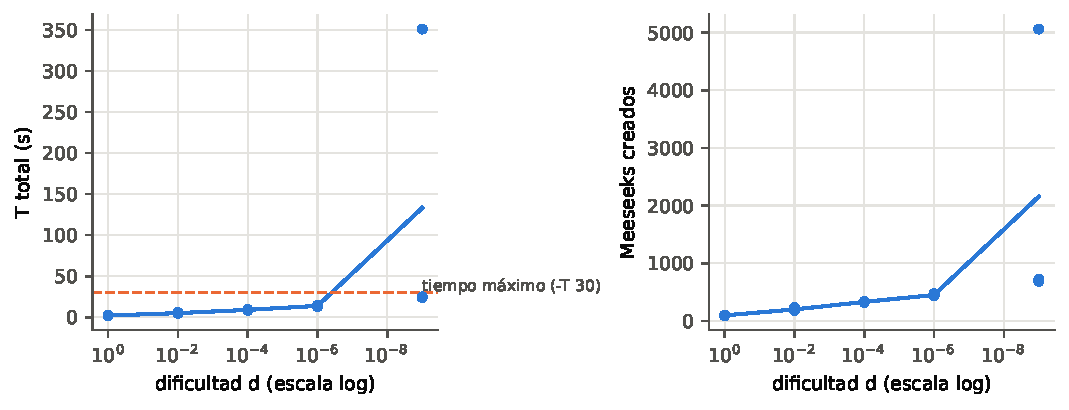
\includegraphics[width=\linewidth]{figs/e6_extra.pdf}
\caption{E6: tiempo total y Meeseeks creados para dificultades muy pequeñas.}
\end{figure}

\paragraph{Observaciones.}
\begin{itemize}[leftmargin=1.5em]
\item Mientras el sistema no se sature, el costo crece de forma logarítmica: cada factor de
  100 en la dificultad agrega unos 5 niveles y unos 4 a 5~s. Incluso $d=10^{-9}$ se resolvió
  en dos de tres corridas en unos 24~s, por debajo del máximo, con unos 700 Meeseeks.
\item La tercera corrida con $d=10^{-9}$ es el caso que pide el enunciado: superó los 30~s,
  se decretó el caos y, sin terminar el programa, la solución llegó a los 351~s, es decir,
  \textbf{321~s adicionales}. Lo notable es que la espera simulada del camino ganador fue de
  solo 22.5~s: casi todo el tiempo (328~s) fue tiempo real del sistema. Se crearon 5059
  Meeseeks, con 4543 vivos a la vez, que consumieron 579~s de CPU en dos núcleos.
\item La explicación es la misma que en E4b. Por azar, ese árbol creció más ancho que los
  otros; con miles de padres esperando un \emph{slot} y reintentando cada 25~ms, la CPU se
  satura en espera activa, los Meeseeks que sí trabajan se planifican tarde y el árbol
  avanza cada vez más lento, lo que a su vez deja más padres esperando. Es una
  retroalimentación positiva: pasado cierto tamaño, la tarea no se vuelve un poco más lenta,
  sino un orden de magnitud más lenta.
\item Conclusión de la prueba: el tiempo adicional que necesita una tarea muy difícil no es
  predecible a partir de su dificultad, porque depende de si el árbol cruza el umbral de
  saturación. Por debajo del umbral bastan segundos; por encima, varios minutos. Esto
  justifica que el tiempo máximo exista y que su acción sea terminar todo el grupo de
  procesos: seguir esperando puede costar mucho más que reintentar la solicitud.
\end{itemize}

A escala real (300~s de máximo y duraciones de 0.5 a 5~s) cada generación tarda en promedio
2.75~s en lugar de 0.25~s, por lo que el mismo árbol necesitaría unas 11 veces más tiempo
simulado: una tarea con $d=10^{-9}$ (unos 34 niveles) pasaría de los 300~s solo por las
esperas, aun sin saturación. Por esa razón la prueba se hizo a escala y no con los 5
minutos completos, que habrían requerido horas por corrida. La terminación por caos con un
tiempo máximo real se muestra en la corrida de la sección~\ref{sec:corridas}.


% ===========================================================================
\section{Conclusiones}

\begin{itemize}[leftmargin=1.5em]
\item Se implementó en un único programa en C la Box de Mr.\ Meeseeks con los tres tipos de
  solicitud. Todos los procesos ejecutan el mismo código, se crean con \texttt{fork()}, se
  comunican solo por pipes y comparten contadores protegidos por semáforos POSIX en memoria
  compartida.
\item La Ley de Dilución logística, con $d=0$ como punto fijo, cumple a la vez dos
  requisitos que parecen opuestos: cualquier tarea posible termina resolviéndose y una
  imposible jamás. Los experimentos muestran que la profundidad crece como $\log(1/d)$ y que
  la cantidad de Meeseeks crece muy rápido al acercarse a 0, como en la serie.
\item La concurrencia trajo problemas reales, no solo teóricos. Varios Meeseeks podían
  resolver la tarea a la vez (se corrigió con una victoria exclusiva en sección crítica) y el
  semáforo de \emph{slots} produjo un interbloqueo que cumplía las cuatro condiciones de
  Coffman (se corrigió liberando el \emph{slot} al pasar a esperar). Ninguno de los dos se
  habría notado sin probar con tareas difíciles.
\item Crear un Meeseeks cuesta unos 0.25~ms y algo menos de 0.2~ms adicionales por cada uno
  en un árbol grande; ejecutar un programa externo cuesta unas 9 veces más por el
  \texttt{exec}. En todas las solicitudes, el tiempo total lo domina la espera simulada,
  por eso el tiempo real debe medirse restando la espera del camino crítico y no la suma de
  todas las esperas.
\item Cuando hay paralelismo, la aleatoriedad ayuda: con duración aleatoria la tarea se
  resolvió antes y con menos procesos, porque gana la rama más rápida.
\item El plan de contingencia funcionó en todas las pruebas: ninguna tarea imposible colapsó
  el sistema. Aun así, la espera por \emph{slots} con sondeo periódico crece en forma
  cuadrática y llega a saturar la CPU con miles de procesos; una espera pasiva sería la
  siguiente mejora.
\item El tiempo máximo no es solo una protección contra tareas imposibles. Las tareas muy
  difíciles pero posibles también pueden superarlo, y entonces terminar el programa
  significa perder una solución que estaba en camino (sección~\ref{sec:e6}). Por eso el
  tiempo máximo es una decisión sobre cuánto se está dispuesto a esperar, y su valor debe
  considerar la profundidad que puede alcanzar el árbol.
\end{itemize}

% ===========================================================================
\begin{thebibliography}{9}
\bibitem{silberschatz} A.~Silberschatz, P.~B.~Galvin y G.~Gagne, \emph{Operating System
  Concepts}, 10.ª ed. Hoboken, NJ, EE.~UU.: Wiley, 2018. Caps.~3 (procesos), 6 y 7
  (sincronización) y 8 (interbloqueos).
\bibitem{blp} N.~Matthew y R.~Stones, \emph{Beginning Linux Programming}, 4.ª ed.
  Indianápolis, IN, EE.~UU.: Wiley, 2008. Caps.~11 (procesos y señales), 13 (comunicación
  entre procesos: pipes) y 14 (semáforos, memoria compartida y colas de mensajes).
\bibitem{kerrisk} M.~Kerrisk, \emph{The Linux Programming Interface}. San Francisco, CA,
  EE.~UU.: No Starch Press, 2010. Caps.~24 a 26 (\texttt{fork}, \texttt{exit},
  \texttt{wait}), 44 (pipes), 53 (semáforos POSIX) y 63 (\texttt{poll}).
\bibitem{coffman} E.~G.~Coffman, M.~Elphick y A.~Shoshani, ``System deadlocks'',
  \emph{ACM Computing Surveys}, vol.~3, n.º~2, pp.~67--78, 1971.
\bibitem{man} The Linux man-pages project, \texttt{fork(2)}, \texttt{pipe(7)},
  \texttt{sem\_overview(7)}, \texttt{poll(2)}, \texttt{prctl(2)}, \texttt{getrusage(2)}.
  [En línea]. Disponible: \url{https://man7.org/linux/man-pages/}
\bibitem{rm} J.~Roiland y D.~Harmon (creadores), ``Meeseeks and Destroy'', \emph{Rick and
  Morty}, temp.~1, ep.~5. Adult Swim, 2014.
\end{thebibliography}
